\documentclass[aspectratio=169, 10pt]{beamer}

% --- Theme & Color Configuration ---
\usetheme{Madrid}
\usefonttheme{professionalfonts}
% \setbeamertemplate{navigation symbols}{}
\setbeamertemplate{headline}{}

% Custom Color Palette
\definecolor{darkslate}{RGB}{30, 41, 59}
\definecolor{lightbg}{RGB}{248, 250, 252}
\definecolor{mathred}{RGB}{192, 41, 43}
\definecolor{accentblue}{RGB}{30, 110, 180}

\definecolor{ulbblue}{RGB}{0, 51, 102}
\definecolor{ulbgold}{RGB}{204, 153, 0}

\setbeamercolor{structure}{fg=ulbblue}
\setbeamercolor{palette primary}{bg=ulbblue, fg=white}
\setbeamercolor{palette secondary}{bg=accentblue, fg=white}
\setbeamercolor{palette tertiary}{bg=darkslate, fg=white}
\setbeamercolor{palette quaternary}{bg=ulbblue, fg=white}
\setbeamercolor{titlelike}{parent=palette primary, fg=white}
\setbeamercolor{frametitle}{bg=ulbblue, fg=white}
\setbeamercolor{block title}{bg=ulbblue!15, fg=ulbblue}
\setbeamercolor{block body}{bg=lightbg, fg=darkslate}
\setbeamercolor{block title alerted}{bg=mathred!15, fg=mathred}
\setbeamercolor{block body alerted}{bg=lightbg, fg=darkslate}
\setbeamercolor{block title example}{bg=accentblue!15, fg=accentblue}
\setbeamercolor{block body example}{bg=lightbg, fg=darkslate}

% --- Additional Packages ---
\usepackage[utf8]{inputenc}
\usepackage[T1]{fontenc}
\usepackage{amsmath, amssymb, amsfonts}
\usepackage{tikz}
\usepackage{pgfplots}
\pgfplotsset{compat=1.18}
\usetikzlibrary{arrows.meta, positioning, calc, patterns}
\usepackage{booktabs}
\usepackage{tcolorbox}

\usepackage{mathtools}  
\mathtoolsset{showonlyrefs} % TO REMOVE QUEATION NUMBERING IF NOT CITED/REFERENCED

% --- Presentation Metadata ---
\title[\textbf{Two-Ray Ground Reflection \& Breakpoint Dynamics}]{\textbf{Two-Ray Multipath Propagation \& Breakpoint Distance}}
\subtitle{Electromagnetic Field Derivation, Asymptotic $d^{-4}$ Law, and Ray-Tracing Engine Validation}
\author[Lucas Placentino]{\textbf{Lucas Placentino}}
\institute[EPB-ULB]{École Polytechnique de Bruxelles - Université libre de Bruxelles}
\date{\textbf{ELEC-H415} (Chapter 3)}

\begin{document}

% =========================================================================
% SLIDE 1: Title Slide
% =========================================================================
\begin{frame}[plain]
    \titlepage
    % \begin{center}
    %     \footnotesize \textcolor{darkslate}{\textbf{Lesson Focus:} Deterministic Physical Channel Modeling (Section 3.1.2)}
    % \end{center}
\end{frame}

% =========================================================================
% SLIDE 2: Context & Physical Motivation
% =========================================================================
\begin{frame}{Physical Propagation: The Failure of Free-Space Friis}
    \begin{columns}[T]
        \begin{column}{0.65\textwidth}
            \textbf{The Free-Space (Friis) Model:}
            \begin{itemize}
                \item Assumes unbounded free space: $P_{RX} \propto d^{-2}$.
                \item In terrestrial or street-canyon links, boundary reflections (ground or lateral walls) are always present.
                \item Friis severely overestimates range (predicting hundreds of kilometers for cellular base stations).
            \end{itemize}
            
            \vspace{0.1cm}
            \begin{block}{Two-Ray Interference}
                The superposition of a direct wave (LOS) and a single specularly reflected wave creates an interference pattern that transitions from an oscillating $d^{-2}$ regime into a steep $d^{-4}$ power falloff.
            \end{block}
        \end{column}
        
        % \begin{column}{0.42\textwidth}
        %     \begin{tcolorbox}[colback=white, colframe=ulbblue, title=\textbf{Lesson Plan}]
        %         \small
        %         \begin{enumerate}
        %             \item \textbf{Electromagnetic Setup:} Vector effective heights \& Thévenin open-circuit induction.
        %             \item \textbf{Rigorous Power Proof:} From antenna currents to gain formulation.
        %             \item \textbf{Boundary \& Paraxial Analysis:} Fresnel reflection at grazing \& 2nd-order Taylor series.
        %             \item \textbf{Asymptotic $d^{-4}$ Derivation:} Proof of frequency independence.
        %             \item \textbf{Breakpoint Distance $d_{BP}$:} Analytical derivation and C++ ray-tracer validation.
        %         \end{enumerate}
        %     \end{tcolorbox}
        % \end{column}
    \end{columns}
\end{frame}

% =========================================================================
% SLIDE 3: Problem Geometry & Electromagnetic Setup
% =========================================================================
\begin{frame}{Two-Ray Geometry \& Image Antenna Principle}
    \begin{columns}[c]
        \begin{column}{0.52\textwidth}
            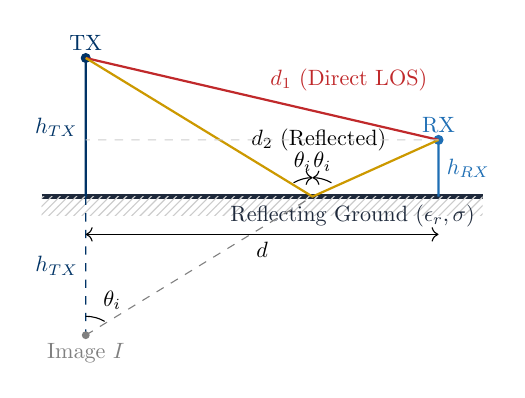
\begin{tikzpicture}[scale=0.8, every node/.style={transform shape}]
                % Reflecting wall / Ground boundary
                \draw[ultra thick, darkslate] (-3.5, 0) -- (3.5, 0);
                \fill[pattern=north east lines, pattern color=gray!40] (-3.5, -0.3) rectangle (3.5, 0);
                \node[below left, darkslate] at (3.5, 0) {Reflecting Ground ($\epsilon_r, \sigma$)};
                
                % Antennas
                \coordinate (TX) at (-2.8, 2.2);
                \coordinate (RX) at (2.8, 0.9);
                \coordinate (Refl) at (0.8, 0);
                \coordinate (Img) at (-2.8, -2.2);
                
                % Heights
                \draw[thick, ulbblue] (-2.8, 0) -- (TX) node[midway, left] {$h_{TX}$};
                \draw[thick, accentblue] (2.8, 0) -- (RX) node[midway, right] {$h_{RX}$};
                \filldraw[ulbblue] (TX) circle (2pt) node[above] {$\text{TX}$};
                \filldraw[accentblue] (RX) circle (2pt) node[above] {$\text{RX}$};
                
                % Rays
                \draw[thick, mathred] (TX) -- (RX) node[midway, above right] {$d_1\text{ (Direct LOS)}$};
                \draw[thick, ulbgold] (TX) -- (Refl) -- (RX);
                \node[above] at (0.9, 0.6) {$d_2\text{ (Reflected)}$};
                
                % Image ray
                \draw[dashed, ulbblue] (-2.8, 0) -- (Img) node[midway, left] {$h_{TX}$};
                \filldraw[gray] (Img) circle (1.5pt) node[below] {Image $I$};
                \draw[dashed, gray] (Img) -- (Refl);
                
                % Distances & Angles
                \draw[dashed, gray!40] (RX) -- (-2.8,0.9);
                \draw[<->] (-2.8, -0.6) -- (2.8, -0.6) node[midway, below] {$d$};
                \draw[->] (0.8, -0.3) ++(120:0.6) arc (120:90:0.6) node[midway, above] {$\theta_i$};
                \draw[->] (0.8, -0.3) ++(60:0.6) arc (60:90:0.6) node[midway, above] {$\theta_i$};
                \draw[-] (-2.8, -2.5) ++(60:0.6) arc (60:90:0.6) node[midway, above right] {$\theta_i$};
            \end{tikzpicture}
        \end{column}
        
        \begin{column}{0.46\textwidth}
            \textbf{Exact Geometric Path Lengths:}
            \begin{align}
                d_1 &= \sqrt{d^2 + (h_{TX} - h_{RX})^2} \label{eq:d1} \\
                d_2 &= \sqrt{d^2 + (h_{TX} + h_{RX})^2} \label{eq:d2} \\
                \theta_i &= \frac{\pi}{2} - \arctan\left(\frac{h_{TX} + h_{RX}}{d}\right) \label{eq:theta_i}
            \end{align}
            \textbf{Hypotheses:}
            \begin{itemize}
                \item 2D propagation in the $xy$-plane.
                \item Linearly polarized electric field normal to the propagation plane ($\vec{E} = E\vec{1}_z$).
                \item Omnidirectional antennas in the plane:
                \begin{equation}
                    \vec{h}_{e\perp}^{TX} = h_{e\perp}^{TX}\vec{1}_z, \quad \vec{h}_{e\perp}^{RX} = h_{e\perp}^{RX}\vec{1}_z
                \end{equation}
            \end{itemize}
        \end{column}
    \end{columns}
\end{frame}

% =========================================================================
% SLIDE 4: Radiated Fields & Open-Circuit Voltage
% =========================================================================
\begin{frame}{Far-Field Radiation \& Induced Open-Circuit Voltage}
    The far-field electric field radiated by the transmitter driven by input current $I_a^{TX}$ at distance $r$ is:
    \begin{equation}
        \vec{E}(\vec{r}) = -j\omega I_a^{TX} \frac{\mu_0}{4\pi} \frac{e^{-j\beta r}}{r} \vec{h}_{e\perp}^{TX}
    \end{equation}
    where $\beta = \frac{2\pi}{\lambda}$ is the free-space wavenumber.

    \begin{columns}[T]
        \begin{column}{0.48\textwidth}
            \begin{block}{1. Direct Wave at Receiver}
                \begin{equation}
                    \vec{E}_1 = -j\omega I_a^{TX} \frac{\mu_0}{4\pi} \frac{e^{-j\beta d_1}}{d_1} h_{e\perp}^{TX} \vec{1}_z
                \end{equation}
            \end{block}
        \end{column}
        \begin{column}{0.48\textwidth}
            \begin{block}{2. Reflected Wave at Receiver}
                \begin{equation}
                    \vec{E}_2 = -j\omega I_a^{TX} \frac{\mu_0}{4\pi} \frac{e^{-j\beta d_2}}{d_2} h_{e\perp}^{TX} \Gamma_\perp(\theta_i) \vec{1}_z
                \end{equation}
            \end{block}
        \end{column}
    \end{columns}

    \vspace{0.2cm}
    \textbf{Open-Circuit Voltage $V_{oc}$ at the RX Terminals:}
    \begin{equation}
        V_{oc} = -\vec{h}_{e\perp}^{RX} \cdot (\vec{E}_1 + \vec{E}_2) 
        = j\omega \frac{\mu_0}{4\pi} I_a^{TX} h_{e\perp}^{TX} h_{e\perp}^{RX} \left[ \frac{e^{-j\beta d_1}}{d_1} + \Gamma_\perp(\theta_i) \frac{e^{-j\beta d_2}}{d_2} \right]
    \end{equation}
\end{frame}

% =========================================================================
% SLIDE 5: Full Analytical Proof: Voltage to Received Power
% =========================================================================
\begin{frame}{Proof: Converting Circuit Voltage into Antenna Gains}
\small
    For a matched receiver ($Z_L = Z_a^*$), the delivered power is $P_{RX} = \frac{1}{8 R_a^{RX}} |V_{oc}|^2$:
    \begin{align}
        P_{RX} &= \frac{|I_a^{TX}|^2}{8 R_a^{RX}} |h_{e\perp}^{TX}|^2 |h_{e\perp}^{RX}|^2 \frac{\omega^2 \mu_0^2}{16\pi^2} \left| \frac{e^{-j\beta d_1}}{d_1} + \Gamma_\perp \frac{e^{-j\beta d_2}}{d_2} \right|^2 \nonumber \\
        &= \underbrace{\left(\frac{1}{2} R_a^{TX} |I_a^{TX}|^2\right)}_{P_{TX}} \cdot \frac{|h_{e\perp}^{TX}|^2}{R_a^{TX}} \frac{|h_{e\perp}^{RX}|^2}{R_a^{RX}} \frac{\omega^2 \mu_0^2}{64\pi^2} \left| \frac{e^{-j\beta d_1}}{d_1} + \Gamma_\perp \frac{e^{-j\beta d_2}}{d_2} \right|^2
    \end{align}
\vspace{-1em}
    \begin{block}{Fundamental Electromagnetic Identities}
        Using $\omega = \beta c = \frac{2\pi c}{\lambda}$, $c^2 \mu_0^2 = Z_0^2$, and the Gain identity $G = \frac{\pi Z_0}{R_a} \frac{|h_{e\perp}|^2}{\lambda^2}$:
        \begin{equation}
            \frac{\omega^2 \mu_0^2}{64\pi^2} \frac{|h_{e\perp}^{TX}|^2}{R_a^{TX}} \frac{|h_{e\perp}^{RX}|^2}{R_a^{RX}} 
            = \left(\frac{\lambda}{4\pi}\right)^2 \underbrace{\left(\frac{\pi Z_0 |h_{e\perp}^{TX}|^2}{\lambda^2 R_a^{TX}}\right)}_{G_{TX}} \underbrace{\left(\frac{\pi Z_0 |h_{e\perp}^{RX}|^2}{\lambda^2 R_a^{RX}}\right)}_{G_{RX}}
        \end{equation}
    \end{block}

    %\textbf{Exact Two-Ray Received Power Equation:}
    \vspace{-1.5em}
    \begin{equation}
        \text{\textbf{Exact Two-Ray Received Power Equation:}}\quad \boxed{P_{RX}(d) = \left(\frac{\lambda}{4\pi}\right)^2 G_{TX} G_{RX} P_{TX} \left| \frac{e^{-j\beta d_1}}{d_1} + \Gamma_\perp(\theta_i) \frac{e^{-j\beta d_2}}{d_2} \right|^2}
    \end{equation}
\end{frame}

% =========================================================================
% SLIDE 6: Boundary Reflection & Grazing Limit
% =========================================================================
\begin{frame}{Fresnel Reflection Coefficient \& The Grazing Limit}
    \begin{columns}[T]
        \begin{column}{0.52\textwidth}
            \textbf{TE Fresnel Reflection Coefficient:}
            \begin{equation}
                \Gamma_\perp(\theta_i) = \frac{\cos\theta_i - \sqrt{\epsilon_r - \sin^2\theta_i}}{\cos\theta_i + \sqrt{\epsilon_r - \sin^2\theta_i}}
            \end{equation}
            where $\epsilon_r$ is the relative permittivity of the reflecting surface (ground here).

            \vspace{0.2cm}
            \begin{alertblock}{Asymptotic Grazing Limit ($d \gg h_{TX}, h_{RX}$)}
                As distance $d$ increases:
                \begin{equation}
                    \theta_i = \frac{\pi}{2} - \arctan\left(\frac{h_{TX} + h_{RX}}{d}\right) \to \frac{\pi}{2}
                \end{equation}
                \begin{equation}
                    \lim_{\theta_i \to \pi/2} \Gamma_\perp(\theta_i) = \frac{0 - \sqrt{\epsilon_r - 1}}{0 + \sqrt{\epsilon_r - 1}} = \mathbf{-1}
                \end{equation}
            \end{alertblock}
        \end{column}
        
        \begin{column}{0.45\textwidth}
            \textbf{Physical Interpretation:}
            \begin{itemize}
                \item At small grazing angle ($\theta_i \to 90^\circ$), our dielectric surface will behave as a \textbf{perfect electrical conductor}.
                \item The reflected wave gets a $\mathbf{180^\circ}$ ($\pi$ rad) phase shift upon reflection ($\Gamma_\perp \to -1$).
                \item The total field becomes a pure \textbf{destructive cancellation problem} controlled entirely by the geometric path difference $\Delta d = d_2 - d_1$.
            \end{itemize}
        \end{column}
    \end{columns}
\end{frame}

% =========================================================================
% SLIDE 7: Paraxial Phase Expansion
% =========================================================================
\begin{frame}{Differential Path $\Delta d = d_2 - d_1$}
\small
    For $d \gg (h_{TX} \pm h_{RX})$, amplitude terms are approximately equal: $d_1 \approx d_2 \approx d$. 
    However, the phase difference $\beta(d_2 - d_1)$ is multiplied by $\beta = \frac{2\pi}{\lambda}$ and must be expanded to second order:

    \begin{align}
        d_1 &= d \sqrt{1 + \left(\frac{h_{TX} - h_{RX}}{d}\right)^2} \simeq d \left[ 1 + \frac{1}{2}\left(\frac{h_{TX} - h_{RX}}{d}\right)^2 \right] = d + \frac{(h_{TX} - h_{RX})^2}{2d} \\
        d_2 &= d \sqrt{1 + \left(\frac{h_{TX} + h_{RX}}{d}\right)^2} \simeq d \left[ 1 + \frac{1}{2}\left(\frac{h_{TX} + h_{RX}}{d}\right)^2 \right] = d + \frac{(h_{TX} + h_{RX})^2}{2d}
    \end{align}

    \begin{block}{Exact Differential Path Difference $\Delta d$}
        Subtracting the two Taylor expansions:
        \begin{equation}
            \Delta d = d_2 - d_1 \simeq \frac{(h_{TX} + h_{RX})^2 - (h_{TX} - h_{RX})^2}{2d} = \frac{4 h_{TX} h_{RX}}{2d} = \mathbf{\frac{2 h_{TX} h_{RX}}{d}}
        \end{equation}
    \end{block}

    \textbf{Differential Phase Shift:}
    \begin{equation}
        \Delta\phi(d) = \beta (d_2 - d_1) \simeq \frac{2\pi}{\lambda} \left(\frac{2 h_{TX} h_{RX}}{d}\right) = \frac{4\pi h_{TX} h_{RX}}{\lambda d}
    \end{equation}
\end{frame}

% =========================================================================
% SLIDE 8: Derivation of the Asymptotic d^-4 Power Law
% =========================================================================
\begin{frame}{Destructive Interference \& Asymptotic $d^{-4}$ Power Law}
\small
    Substituting $\Gamma_\perp \simeq -1$ and $d_1 \approx d_2 \approx d$ into {\footnotesize$P_{RX}(d) = \left(\frac{\lambda}{4\pi}\right)^2 G_{TX} G_{RX} P_{TX} \left| \frac{e^{-j\beta d_1}}{d_1} + \Gamma_\perp(\theta_i) \frac{e^{-j\beta d_2}}{d_2} \right|^2$}
    \begin{align}
        P_{RX} &\simeq \left(\frac{\lambda}{4\pi}\right)^2 \frac{G_{TX} G_{RX} P_{TX}}{d^2} \left| e^{-j\beta d_1} - e^{-j\beta d_2} \right|^2 \nonumber \\
        &= \left(\frac{\lambda}{4\pi}\right)^2 \frac{G_{TX} G_{RX} P_{TX}}{d^2} \left| 1 - e^{-j\beta(d_2 - d_1)} \right|^2 
        = 4 \left(\frac{\lambda}{4\pi}\right)^2 \frac{G_{TX} G_{RX} P_{TX}}{d^2} \sin^2\left(\frac{\beta(d_2 - d_1)}{2}\right)
    \end{align}

    \begin{block}{Small-Angle Taylor Approximation for $d \to \infty$}
        Since $\frac{\beta(d_2 - d_1)}{2} = \frac{\beta h_{TX} h_{RX}}{d} \ll 1$, we use $\sin(x) \simeq x$:
        \begin{equation}
            \sin^2\left(\frac{\beta h_{TX} h_{RX}}{d}\right) \simeq \left(\frac{\beta h_{TX} h_{RX}}{d}\right)^2 = \left(\frac{2\pi}{\lambda} \frac{h_{TX} h_{RX}}{d}\right)^2
        \end{equation}
    \end{block}

    \textbf{Final Asymptotic Power Law (Complete Cancellation of Wavelength $\lambda$):}
    \begin{equation}
        P_{RX}(d) \simeq 4 \left(\frac{\lambda}{4\pi}\right)^2 \frac{G_{TX} G_{RX} P_{TX}}{d^2} \cdot \frac{4\pi^2 h_{TX}^2 h_{RX}^2}{\lambda^2 d^2} 
        \implies \boxed{P_{RX}(d) = G_{TX} G_{RX} P_{TX} \frac{h_{TX}^2 h_{RX}^2}{d^4}}
    \end{equation}
\end{frame}

% =========================================================================
% SLIDE 9: Analytical Derivation of the Breakpoint Distance
% =========================================================================
\begin{frame}{Analytical Derivation of the Breakpoint Distance $d_{BP}$}
\small
    The propagation profile exhibits two fundamental regimes separated by a **breakpoint**:
    \begin{itemize}
        \item \textbf{Near Region ($d \le d_{BP}$):} Constructive/destructive interference ripples around Friis loss ($n = 2$).
        \item \textbf{Far Region ($d > d_{BP}$):} Monotonic destructive cancellation with steep roll-off ($n = 4$).
    \end{itemize}

    \begin{block}{Friis and Asymptotic Power Envelopes}
        The transition distance $d_{BP}$ occurs where the asymptotic $d^{-4}$ curve intersects Friis free-space power:
        \begin{equation}
            P_{RX, \text{Friis}}(d_{BP}) = P_{RX, \text{asympt}}(d_{BP})
        \end{equation}
        \begin{equation}
            G_{TX} G_{RX} P_{TX} \left(\frac{\lambda}{4\pi d_{BP}}\right)^2 = G_{TX} G_{RX} P_{TX} \frac{h_{TX}^2 h_{RX}^2}{d_{BP}^4}
        \end{equation}
        \begin{equation}
            \frac{\lambda^2}{16\pi^2 d_{BP}^2} = \frac{h_{TX}^2 h_{RX}^2}{d_{BP}^4} \implies d_{BP}^2 = \frac{16\pi^2 h_{TX}^2 h_{RX}^2}{\lambda^2}
        \end{equation}
    \end{block}

    \textbf{The Analytical Breakpoint Distance:}
    \begin{equation}
        \boxed{d_{BP} = \frac{4\pi h_{TX} h_{RX}}{\lambda} = \frac{4\pi f h_{TX} h_{RX}}{c}}
    \end{equation}
\end{frame}

% =========================================================================
% SLIDE 10: Spatial Fading Dynamics & Null Distribution
% =========================================================================
% \begin{frame}{Spatial Fading Pitch in the Near Region ($d < d_{BP}$)}
%     In the interference region, destructive nulls occur whenever the phase difference equals an odd multiple of $\pi$:
%     \begin{equation}
%         \Delta\phi = \frac{4\pi h_{TX} h_{RX}}{\lambda d} = (2m - 1)\pi \quad (m \in \mathbb{N}^+)
%     \end{equation}

%     \begin{columns}[T]
%         \begin{column}{0.50\textwidth}
%             \begin{block}{Exact Null Locations $d_m$}
%                 \begin{equation}
%                     d_m = \frac{4 h_{TX} h_{RX}}{(2m - 1)\lambda}
%                 \end{equation}
%                 The final destructive null ($m = 1$) occurs at:
%                 \begin{equation}
%                     d_{\text{last null}} = \frac{4 h_{TX} h_{RX}}{\lambda} = \frac{d_{BP}}{\pi} \approx \mathbf{0.318 \, d_{BP}}
%                 \end{equation}
%             \end{block}
%         \end{column}
        
%         \begin{column}{0.48\textwidth}
%             \textbf{Spatial Fringe Pitch $\delta d$:}
%             \begin{equation}
%                 \delta d \approx \left| \frac{\partial d_m}{\partial m} \right| \simeq \frac{\lambda d^2}{2 h_{TX} h_{RX}}
%             \end{equation}
%             \begin{itemize}
%                 \item Close to the transmitter ($d \ll d_{BP}$), nulls are extremely close together ($\delta d \sim \text{cm}$ or $\text{mm}$).
%                 \item As $d \to d_{BP}$, the fringe spacing expands until the last null is reached.
%             \end{itemize}
%         \end{column}
%     \end{columns}
% \end{frame}

% =========================================================================
% SLIDE 11: Project Validation: Single-Reflection Ray-Tracing Engine
% =========================================================================
\begin{frame}{Ray-Tracing Engine Validation (Project Results)}
    \begin{columns}[c]
        \begin{column}{0.58\textwidth}
        \begin{figure}
            \centering
            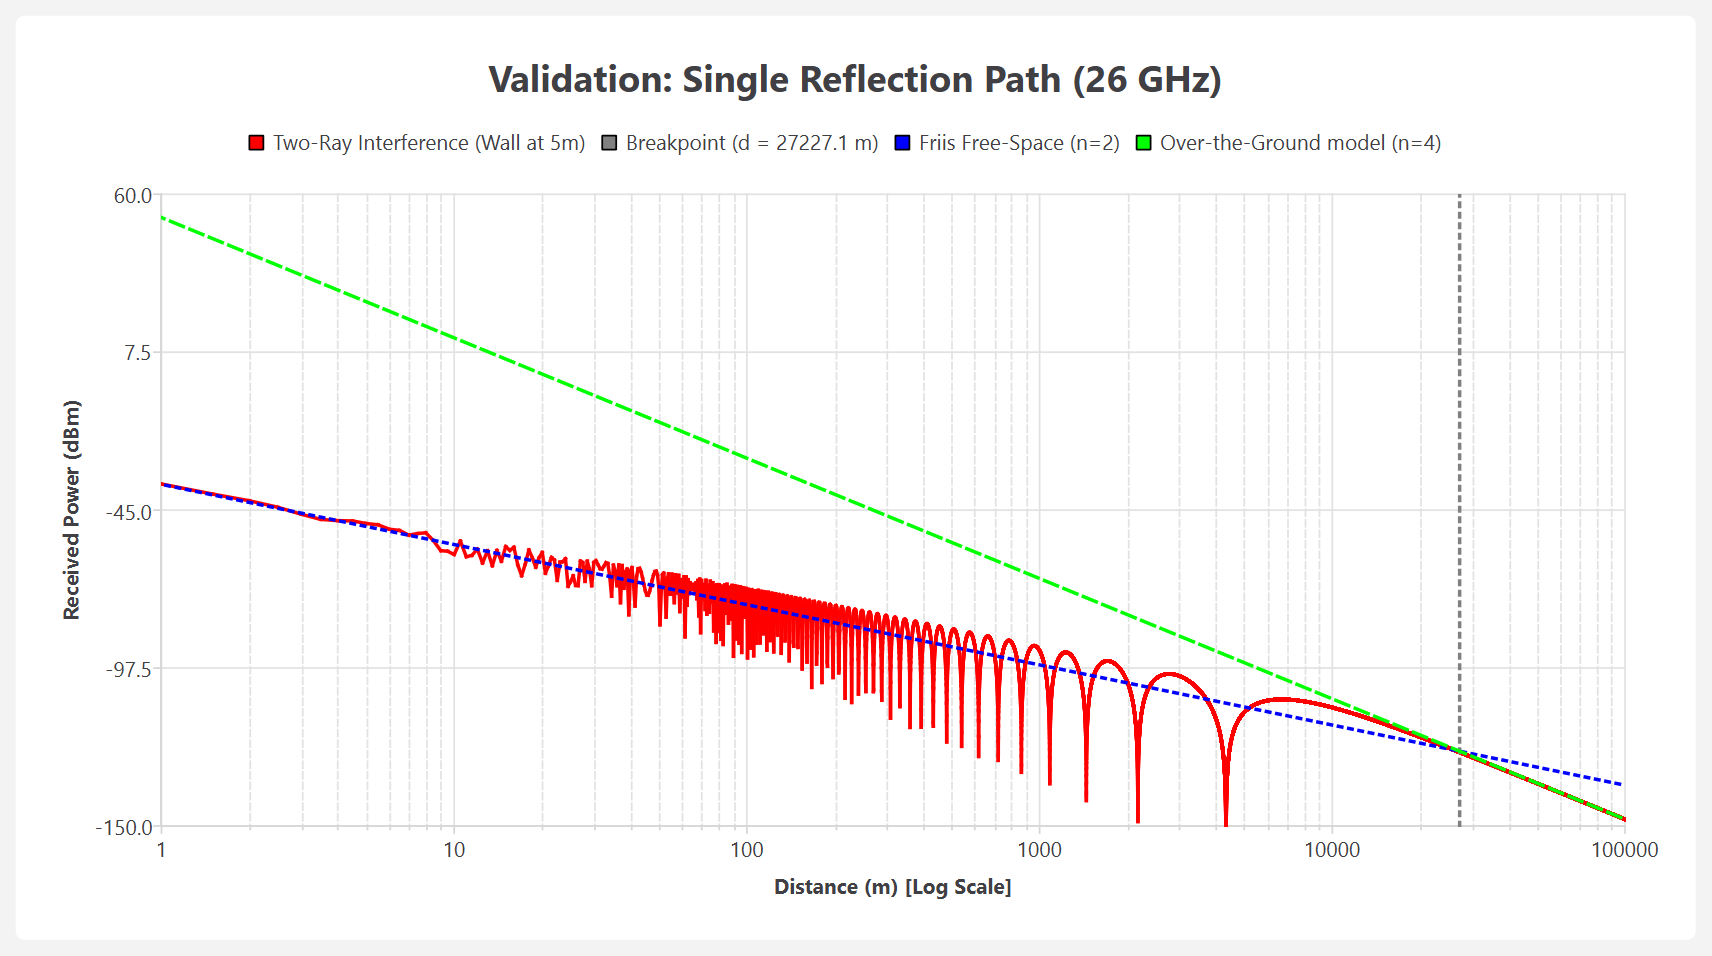
\includegraphics[width=1\linewidth]{image.png}
            %\caption{Enter Caption}
            %\label{fig:placeholder}
        \end{figure}
            % \begin{tikzpicture}[scale=0.75]
            %     \begin{axis}[
            %         xmode=log,
            %         xlabel={Distance $d$ [m] (Log Scale)},
            %         ylabel={$P_{RX}$ [dBm]},
            %         xmin=1, xmax=100000,
            %         ymin=-150, ymax=0,
            %         grid=both,
            %         major grid style={line width=.2pt,draw=gray!30},
            %         width=8.5cm, height=6.0cm,
            %         legend pos=north east,
            %         legend style={font=\tiny}
            %     ]
            %         % Friis Line (n=2)
            %         \addplot[domain=1:100000, samples=50, line width=1.2pt, green!60!black] 
            %             {-20 - 20*log10(x)};
            %         \addlegendentry{Friis Free-Space ($n=2$)}
                    
            %         % Asymptotic Line (n=4)
            %         \addplot[domain=5000:100000, samples=50, line width=1.2pt, red!80!black] 
            %             {10*log10(10^(-2.0) * (20*20)^2 / (x^4))};
            %         \addlegendentry{Over-the-Ground ($n=4$)}
                    
            %         % Simulated Single-Reflection Ray Trace (Project Engine)
            %         \addplot[domain=1:100000, samples=400, thick, blue] 
            %             {-20 - 20*log10(x) + 10*log10(4*(sin(deg(2*pi*20*20/(0.0115*x))))^2 + 0.00001)};
            %         \addlegendentry{Simulated Two-Ray (26 GHz)}
                    
            %         % Breakpoint Marker
            %         \draw[dashed, black, thick] (axis cs:27227, -150) -- (axis cs:27227, 0);
            %         \node[above left, font=\tiny, rotate=90] at (axis cs:27227, -120) {$d_{BP} = 27\,227\text{ m}$};
            %     \end{axis}
            % \end{tikzpicture}
        \end{column}
        
        \begin{column}{0.40\textwidth}
            \begin{tcolorbox}[colback=white, colframe=ulbblue, title=\textbf{Validation Scene (App. A.2)}]
                \centering
                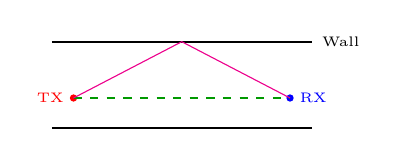
\begin{tikzpicture}[scale=0.55]
                    \draw[thick] (-3,1) -- (3,1) node[right, font=\tiny] {Wall};
                    \draw[thick] (-3,-1) -- (3,-1);
                    \filldraw[red] (-2.5, -0.3) circle (2pt) node[left, font=\tiny] {TX};
                    \filldraw[blue] (2.5, -0.3) circle (2pt) node[right, font=\tiny] {RX};
                    \draw[green!60!black, dashed] (-2.5, -0.3) -- (2.5, -0.3);
                    \draw[magenta] (-2.5, -0.3) -- (0, 1) -- (2.5, -0.3);
                \end{tikzpicture}
            \end{tcolorbox}
            \footnotesize
            \textbf{Simulation Setup ($26\text{ GHz}$):}
            \begin{itemize}
                \item $h_{TX} = h_{RX} = w = 5\text{ m}$, $\lambda = 1.15\text{ cm}$.
                \item $d_{BP} = \frac{4\pi (5)^2}{0.0115} = \mathbf{27\,227\text{ m}}$.
                \item Verifies the $n=2 \to n=4$ transition and asymptotic convergence!
            \end{itemize}
        \end{column}
    \end{columns}
\end{frame}

% =========================================================================
% SLIDE 12: Applied Engineering Takeaways: Sub-6 GHz vs. mmWave
% =========================================================================
\begin{frame}{Applied System Takeaways: Sub-6\,GHz vs. mmWave 5G}
    \begin{exampleblock}{Breakpoint Scaling Across 5G Operating Bands}
        Consider a street-level small cell where $h_{TX} = 4\text{ m}$ (lamppost) and $h_{RX} = 1.5\text{ m}$ (pedestrian UE):
    \end{exampleblock}

    \begin{table}[h]
        \centering
        \small
        \footnotesize
        \begin{tabular}{lcccc}
            \toprule
            \textbf{5G Band} & \textbf{Frequency ($f$)} & \textbf{Wavelength ($\lambda$)} & \textbf{Breakpoint ($d_{BP}$)} & \textbf{Physical Regime in Cell ($R \le 150\text{m}$)} \\
            \midrule
            \textbf{Low-Band} & $700\text{ MHz}$ & $42.8\text{ cm}$ & $\mathbf{176\text{ m}}$ & Reaches $n=4$ asymptotic decay at cell edge \\
            \textbf{Mid-Band} & $3.5\text{ GHz}$ & $8.57\text{ cm}$ & $\mathbf{880\text{ m}}$ & Near-breakpoint transition zone \\
            \textbf{mmWave} & $26\text{ GHz}$ & $1.15\text{ cm}$ & $\mathbf{6.54\text{ km}}$ & \textbf{Strictly $n=2$ with fast multipath ripples} \\
            %\textbf{WiGig / V-Band} & $60\text{ GHz}$ & $5.0\text{ mm}$ & $\mathbf{15.08\text{ km}}$ & \textbf{Strictly $n=2$ with fast multipath ripples} \\
            \bottomrule
        \end{tabular}
    \end{table}

    \begin{alertblock}{Design Consequence for mmWave}
        \begin{itemize}
            \item At $26\text{ GHz}$, small cells ($R \ll d_{BP}$) never enter the $d^{-4}$ region.
            %\item The main challenge is not ground roll-off, but \textbf{millimeter-scale interference nulls}, mitigated using **narrow beamforming** that spatially filters out the ground/wall bounce.
        \end{itemize}
    \end{alertblock}
\end{frame}

% =========================================================================
% SLIDE 13: Summary & Key Takeaways
% =========================================================================
\begin{frame}{Summary of Mathematical \& Physical Results}
    \begin{block}{1. Complete Theoretical Derivation Chain}
        \begin{equation*}
            V_{oc} = -\vec{h}_{e\perp}\cdot\vec{E}_{tot} \xrightarrow{\text{Matched Load}} P_{RX} = \left(\frac{\lambda}{4\pi}\right)^2 G_{TX} G_{RX} P_{TX} \left| \frac{e^{-j\beta d_1}}{d_1} + \Gamma_\perp \frac{e^{-j\beta d_2}}{d_2} \right|^2
        \end{equation*}
        \begin{equation*}
            \xrightarrow[d \gg h_{TX}, h_{RX}]{\Gamma_\perp \to -1, \; \Delta d \simeq \frac{2 h_{TX} h_{RX}}{d}} \boxed{P_{RX}(d) = G_{TX} G_{RX} P_{TX} \frac{h_{TX}^2 h_{RX}^2}{d^4}} \quad \text{(\textbf{Frequency Independent!})}
        \end{equation*}
    \end{block}

    \begin{columns}[T]
        \begin{column}{0.48\textwidth}
            \begin{block}{2. The Breakpoint Distance}
                $$\boxed{d_{BP} = \frac{4\pi h_{TX} h_{RX}}{\lambda} = \frac{4\pi f h_{TX} h_{RX}}{c}}$$
                Marks the boundary where ground cancellation permanently sets in.
            \end{block}
        \end{column}
        
        \begin{column}{0.48\textwidth}
            \begin{block}{3. Simulation Validation}
                The 2D C++ ray-tracer strictly confirms:
                \begin{itemize}
                    \item Ripple dynamics for $d < d_{BP}$.
                    \item Exact $n=4$ asymptotic slope for $d > d_{BP}$.
                \end{itemize}
            \end{block}
        \end{column}
    \end{columns}
\end{frame}

\end{document}